\documentclass{beamer}

\title{Tutorial 1}
\subtitle{Intro, Intro, Intro}

%\usetheme{lucid}
\begin{document}
	\frame {
		\titlepage
	}
	
	\begin{frame}{TA Intro:}
		\begin{itemize}
			\item Name: Zayd
			\item OH: Thursday 10:00 am - 11:00 am or by appointment if this time doesn't work
			\item email: zayd.omar@mcgill.ca
			\item About me: I'm a $1^{st}$ year PhD student.
		\end{itemize}
	\end{frame}
	
	\begin{frame}{Tutorial Intro:}
		\begin{itemize}
			\item The \textbf{main} goal of the tutorials is to \textbf{practice problems} and get \textbf{training} in $\mathtt{R}$.
			\item Only have about 50-60 mins every week to cover most of the material (and other extra stuff for the assignments)
			\item Ideally, I would like to structure the tutorial so that, we spend 5-10 mins quickly reviewing over the materials covered in class.
			\item The rest of the time we want to spend solving a few problems from the book and also figuring out the $\mathtt{R}$ stuff which you will need in your assignments.
			\item Although this is \textbf{NOT} a requirement, I encourage everyone to learn LaTeX and to type up your assignments. This is a super useful skill to have for anyone who is in STEM and in the medical field. 
			\item I'm happy to help you learn LaTeX alongside learning $\mathtt{R}$.
		\end{itemize}
	\end{frame}
	
	\begin{frame}{$\mathtt{R}$ Intro:}
		\begin{itemize}
			\item First thing to do is to download $\mathtt{R}$, from the CRAN website.
			\item The mirror you use is not important. (I think I most recently used the Toronto mirror.) \\
			\vspace{4pt}
			$https://utstat.toronto.edu/cran/$ \\
			\vspace{5pt}
			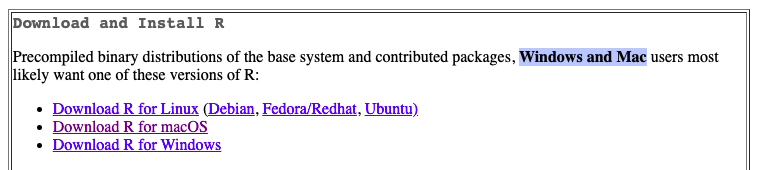
\includegraphics[width=10cm,height=2cm]{pic1.png}
			\vspace{4pt}
			\item Choose the $\mathtt{R}$ version based on your laptop/PC specifications. 
			\item Install $\mathtt{R}$ to your computer.
			\item You can now run $\mathtt{R}$ as is and do most of your work, but we will take one extra step that will make  $\mathtt{R}$ \textbf{MUCH MORE} user friendly.
		\end{itemize}
	\end{frame}
	
	\begin{frame}{$\mathtt{R}$-Studio:}
		\begin{itemize}
			\item Download, $\mathtt{R}$-Studio from, https://www.rstudio.com/products/rstudio/download/
			\item Choose the free version, RStudio Desktop. We don't need anything fancy.
			\item RStudio provides a better and more convenient user interface than $\mathtt{R}$.
			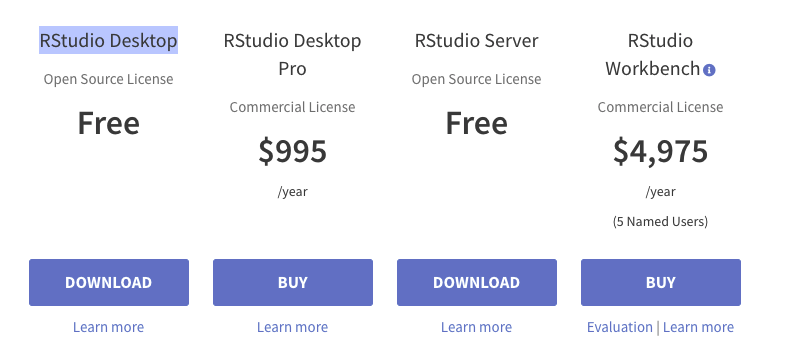
\includegraphics[width=10cm,height=4cm]{pic2.png}
			\item \textbf{Note:} Install $\mathtt{R}$ before you install RStudio otherwise there might be some problems.
			
		\end{itemize}
	\end{frame}
	
	
	\begin{frame}{Basic R-Functions}
		\begin{itemize}
			\item (See attahced $\mathtt{R}$ code, named $\mathtt{R\_Script\_1}$)
			\item We need to be able import $\mathtt{.csv}$ files in to $\mathtt{R}$.
			\item Using basic arithmetic functions, in particular vectorization techniques in $\mathtt{R}$.
			\item Using basic statistical commands for mean, variance, p-values.
			\item Using basic plot functions for, histograms, 2-d scatter plots, QQ-plots.
		\end{itemize}
	\end{frame}
	\begin{frame}{Some Exercises:}
		\begin{itemize}
			\item Import the data set, $\mathtt{Temp\_Data.csv}$,  provided in MyCourses into R.
			\item Try accessing some of the different variables available.
			\item Find the mean, variance and standard deviation of temperature (and any other variable you wish).
			\item Make scatter plots and histograms on the temperature variable.
			\item Investigate vectorization in $\mathtt{R}$: vector-vector multiplications, vector-scalar multiplications, vector transformations. (These will help us later for some of the regression stuff.)
		\end{itemize}
	\end{frame}
	\begin{frame}{Review of MATH 203:}
		\begin{itemize}
			\item Those of you coming from MATH 203, already have the installation part covered.
			\item Those of you who still have some problems let me know we'll resolve it together.
			\item MATH 203 covered some of the basic introductory stuff in inferential statistics.
			\item You don't need to remember everything off the top of your head, but we really want to remember some things from the second half of the course such as, normal distribution, confidence intervals and hypothesis testing.
			\item We will use these ideas freely in our study of regression.
			\item Other than that the math/stats requirement to be successful in this course is fairly minimal.
		\end{itemize}
	\end{frame}
	
	
	
	
	
	\begin{frame}{Review: Simple Linear Regression}
		\begin{itemize}
			\item We want to model the following linear relationship, $y_i=\beta_0+\beta_1x_i+\epsilon_i$, where $i=1,...,n$.
			\item \textbf{Assumptions}: $\epsilon_i$ are i.i.d with mean $0$ and variance $\sigma^2$.
			\item \textbf{Method:} We use the least squares method.
			\item \textbf{Intuition:} What are we modeling? We are modeling the \textbf{mean response} of $Y$, i.e. we are modeling $E(y_i)=\beta_0+\beta_1x_i$.
			\item \textbf{Check:} Is the relationship linear? Plot the data to check
			\item Simple linear regression can be easily done by hand (although this might be painstakingly slow to do given the sample size).
			\item Ideally, we will do all of our calculation on a software.
		\end{itemize}
	\end{frame}
	
	
	\begin{frame}{Formulas}
		\begin{itemize}
			\item Parameter estimates,
			\begin{align*}
				\begin{split}
					\hat{\beta}_1 &= \frac{S_{xy}}{S_{xx}}=\frac{\sum^n_{i=1} (x_i-\bar{x})(y_i-\bar{y})}{ \sum^n_{i=1}  (x_i-\bar{x})^2}\\
					\hat{\beta}_0 &= \bar{y}-\hat{\beta}_1\bar{x} 
				\end{split}
			\end{align*}
			
			\item Variance of the estimators,
			
			\begin{align*}
				\begin{split}
					\sigma^2_{\hat{\beta}_1} &= \frac{\sigma^2}{S_{xx}}\\
					\sigma^2_{\hat{\beta}_0} &= \sigma^2 \Big(\frac{1}{n}+\frac{\bar{x}^2}{S_{xx}}\Big)
				\end{split}
			\end{align*}
			\item Estimate of variance, $$\hat{\sigma}^2=\frac{SSE}{n-2}$$
			
		\end{itemize}
	\end{frame}
	
	\begin{frame}{Example 1: Some essential calculations and simplifications}
		\begin{itemize}
			\item Show $\sum_{i=1}^n (x_i-\bar{x})^2 = \sum_{i=1}^n x_i^2- n\bar{x}^2$
			\item Show a similar result for $\sum_{i=1}^n (y_i-\bar{y})^2$
			\item Show $\sum_{i=1}^n (x_i-\bar{x})(y_i-\bar{y}) = \sum_{i=1}^n x_iy_i- n\bar{x}\bar{y}$
			\item You'll soon see how these results will help in calculating the regression results in the next problem.
		\end{itemize}
	\end{frame}
	
	
	\begin{frame}{Example 2: (If time permits)}
		\begin{itemize}
			\item Using the $\mathtt{Temp\_Data.csv}$ data, regress $Force$ on $Temp$.
			\item Show in details how the coefficients are calculated.
		\end{itemize}
	\end{frame}
	
\end{document}